\chapter*{Appendix B: Database}
\section*{Hovedvindue for serveren}
\begin{figure}[htbp]
	\centering
	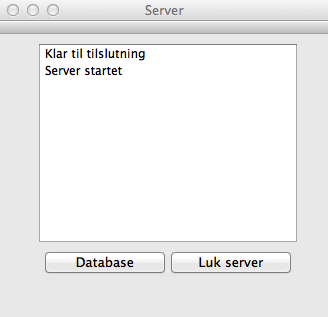
\includegraphics[width=0.4\textwidth]{billeder/database/server}
	\caption{Billed af serverens hovedvindue}
	\label{fig:server}
\end{figure}
Severens GUI giver mulighed for at brugeren kan se at serveren køre og vilke kommandoer der er blevet udført. Fra serverens hovedmodul har brugeren mulighed for at vælge at åbne den den web baserede database og lukke severen.
\begin{table}[H]
\begin{tabular}{l p{12.5cm}}
\multicolumn{2}{l}{Hovedvinduets elementer} \\
\hline
\textcolor{green}{\textbf{1: Info}}
&Brugeren får her udskrevet beskeder om serveren. Brugeren kan se om KI har tilsluttet sig og om der er blevet overført data desuden vil fejl meddelelser blive udskrevet her. Dialog boksen er lavet sådan at den nyeste besked altid står øverst se \ref{fig:server_on}\\

\textcolor{blue}{\textbf{2: Database}}
&Anvendes til at lade brugeren tilgå den web baserede database som ses i \ref{fig:web_pass}\\

\textcolor{red}{\textbf{2: Luk serveren}}
&Anvendes til at lukke programmet. Programmet åbner dialogen som ses i \ref{fig:databselLogOff}\\

\end{tabular}
\end{table}

\begin{figure}[htbp]
	\centering
	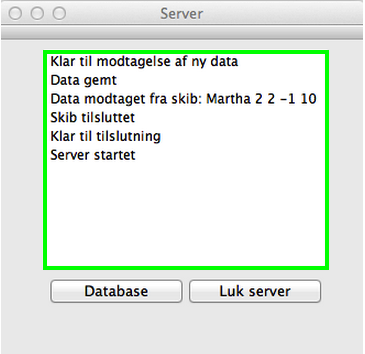
\includegraphics[width=0.4\textwidth]{billeder/database/server_on}
	\caption{Billed af serverens hovedvindue}
	\label{fig:server_on}
\end{figure}


\subsection*{Luk Severen}
\begin{figure}[H]
	\centering
	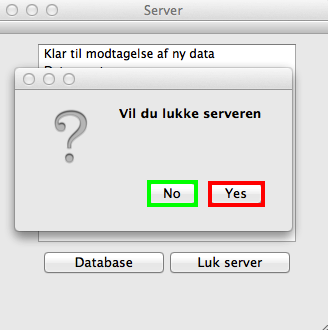
\includegraphics[width=0.4\textwidth]{billeder/database/databaseLogOff}
	\caption{Luk server}
	\label{fig:databselLogOff}
\end{figure}
Ved tryk på "Luk server" vil billedet \ref{fig:databselLogOff} fremkomme og man kan trykke "Yes" for for at lukke severen og "No" for at lade severen fortsætte med at køre.

\begin{table}[H]
\begin{tabular}{l p{12.5cm}}
\multicolumn{2}{l}{Lukke sekvens} \\
\hline
\textcolor{green}{\textbf{1: Info}}
&Ved tryk på "No" vil brugeren retunere til \ref{fig:hovedvindue} og fortsætte med at modtage data fra KI\\

\textcolor{red}{\textbf{2: Luk serveren}}
&Ved tryk på "Yes" vil serveren blive lukket og brugeren kan ikke længere modtage data fra KI.\\

\end{tabular}
\end{table}


\section*{Webside}
\subsection*{Log on}
Den web baserede adgang til databasen
\begin{figure}[H]
	\centering
	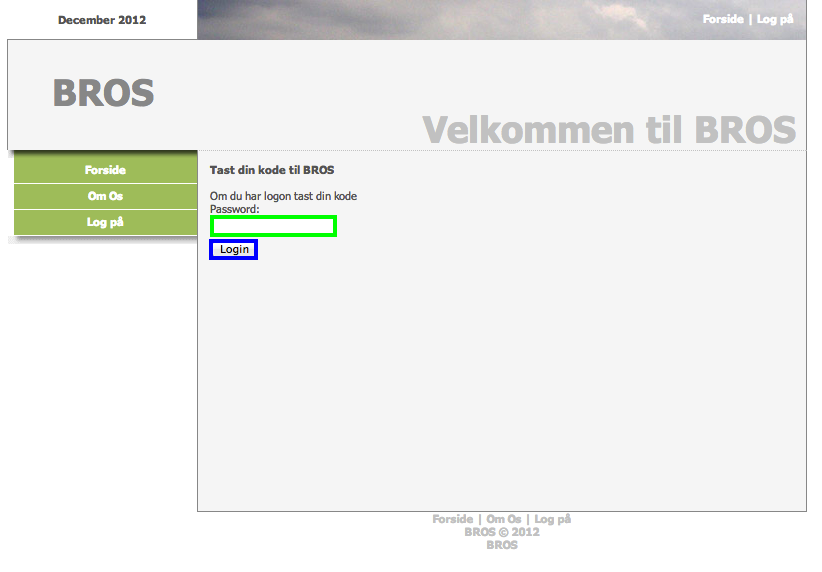
\includegraphics[width=0.8\textwidth]{billeder/database/web_pass}
	\caption{Billed af log in på den web baserede database}
	\label{fig:web_pass}
\end{figure}

\begin{table}[H]
\begin{tabular}{l p{12.5cm}}
\multicolumn{2}{l}{Password check for adgang til den web baserede database } \\
\hline
\textcolor{green}{\textbf{1: Password check}}
&Når brugeren åbner databasen fra serveren vil denne komme til den web baserede database. For at få adgang til databasen skal brugeren taste det password som er blevet opgivet til denne\\
\end{tabular}
\end{table}

\subsection*{Skibs valg}
Efter log in kan brugeren vælge imellem de skibe der er i dennes database. I dette tilfælde findes der kun et skib "Martha".
\begin{figure}[H]
	\centering
	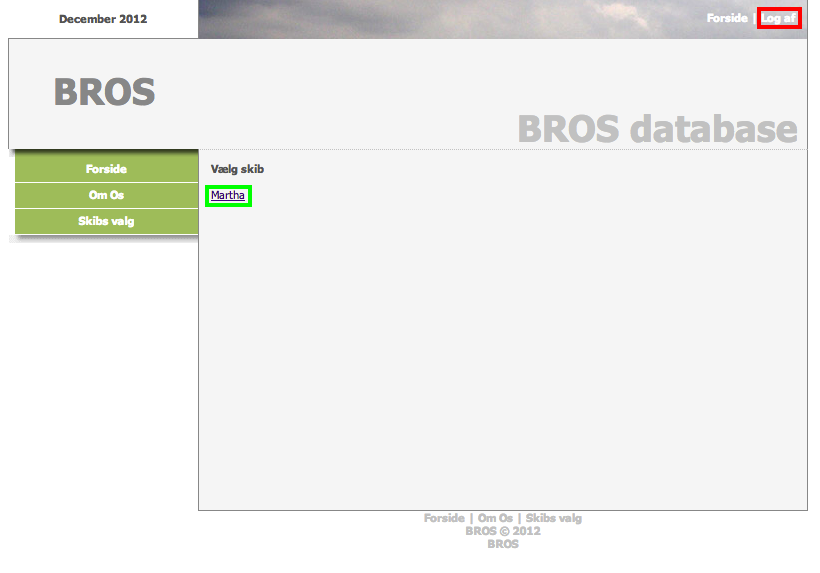
\includegraphics[width=0.8\textwidth]{billeder/database/web_ship_choice}
	\caption{Billed efter log in på databasen. Her kan brugeren vælge skib}
	\label{fig:web_ship_choice}
\end{figure}

\begin{table}[H]
\begin{tabular}{l p{12.5cm}}
\multicolumn{2}{l}{Valg af skib der vil tilgås } \\
\hline
\textcolor{green}{\textbf{1: Valg af skib}}
&Efter at brugeren er logget på som på \ref{fig:web_pass} kan brugeren vælge imellem de skibe som denne har adgang til fra sin database del. Fo havne kontoret ville dette normalt være alle skibe. I denne test version er der kun et skib "Martha"\\
\textcolor{red}{\textbf{2: Log af}}
&Efter at brugeren er logget ind vil denne på alle sider have mulighed for at logge af, dette sker ved at trykke på Log af.\\
\end{tabular}
\end{table}

\subsection*{Skibs data i database}
Efter at brugeren har valgt skib kan denne følge med i tilstanden på skibet. Denen side opdateres hver 5 secund hvis der er ny data.
\begin{figure}[H]
	\centering
	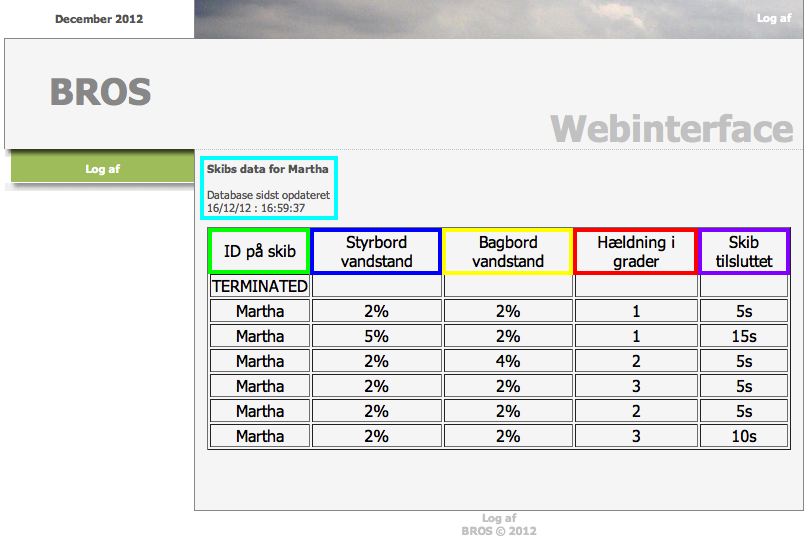
\includegraphics[width=0.8\textwidth]{billeder/database/web_database}
	\caption{Billed databasen BROS for skibet Martha}
	\label{fig:web_database}
\end{figure}
\begin{table}[H]
\begin{tabular}{l p{12.5cm}}

\multicolumn{2}{l}{Data fra skib i databasen } \\
\hline
\textcolor{Turquoise}{\textbf{1: Skib og sidst opdateret}}
&Brugeren kan se hvilket skib denne er inde på og hvornår databasen sidst er opdateret.\\
\textcolor{green}{\textbf{2: ID på skib}}
&Skibets ID bliver vidst. Hvis at KI lukker tcp forbindelsen vil skibts ID skifte til "TERMINATED".\\
\textcolor{blue}{\textbf{3: Styrbord vandtanksniveau}}
&Der vises hvor meget vand der er i styrbord ballasttank.\\
\textcolor{yellow}{\textbf{4: Bagbord vandtanksniveau}}
&Der vises hvor meget vand der er i bagbord ballasttank.\\
\textcolor{red}{\textbf{5: Hældning i grader}}
&Der vises hvor mange grader sibet hælder i forhold til styrbord.\\
\textcolor{RoyalPurple}{\textbf{6: Skib tilsluttet}}
&Der vise hvor lang tid i secunder der er gået fra overførelsen før til denne.\\
\end{tabular}
\end{table}

\subsection*{BROS forside}
Om ikke at brugeren tilgår BROS databasen fra serveren vil forsiden fremkomme, denne kan også tilgås fra databasen.
\begin{figure}[H]
	\centering
	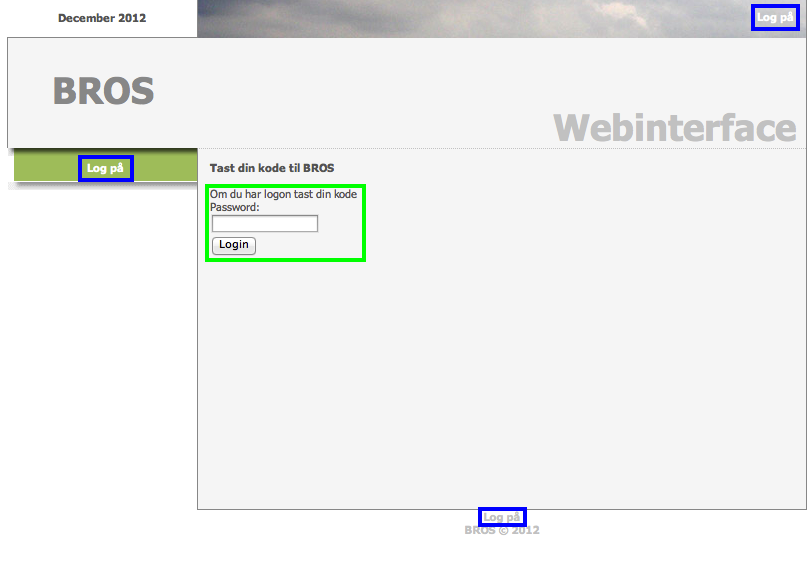
\includegraphics[width=0.8\textwidth]{billeder/database/web_forside}
	\caption{Billed BROS forside}
	\label{fig:web_forside}
\end{figure}

\subsection*{Om BROS}
Efter at brugeren har valgt skib kan denne følge med i tilstanden på skibet. Denen side opdateres hver 5 secund hvis der er ny data.
\begin{figure}[H]
	\centering
	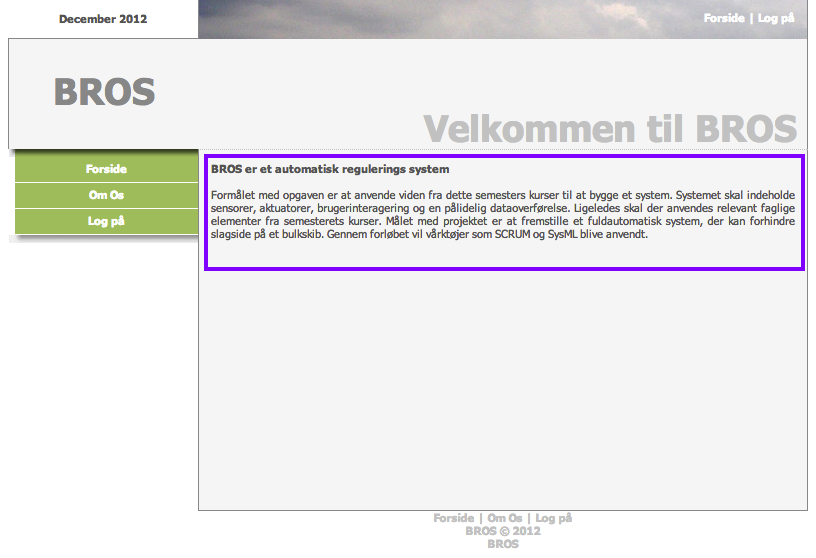
\includegraphics[width=0.8\textwidth]{billeder/database/web_about}
	\caption{Billed af om os på web siden}
	\label{fig:web_about}
\end{figure}


\section*{MySQL}
MySQL er en flertrådet SQL-database som understøtter mange samtidige brugere. MySQL er en open-source program som kan downloades på mysql.com og kan benyttes med mange forskellige operativ systemer som f.eks. WIndows, Linux og MAC OS X Lion.
Under projektet er mySQL blevet benyttet på Ubuntu(Linux version) og MAC OS X Lion. TIlgang til denne er blevet gjort med den grafiske bruger grænseflade phpMyAdmin (webbaseret) og terminalen\footnote{beskrevet under afsnittet: Kommandoer for adgang og brug af mySQL i terminal}

\subsection*{Datatyper}
MySQL understøtte følgende datatyper\footnote{Kilde mysql.com} \\
\textbf{INT} -familien:\\
\textbf{INT}: Bruges udelukkende til heltal som ikke indeholder mellemrum, linjeskift eller lignende.\\
\textbf{SmallINT}: Fungere som INT, men bruges til små tal.\\
\textbf{MediumINT}: Fungere som INT, men bruges til mellemstore tal.\\
\textbf{BigINT}: Fungere som INT, men bruges til store tal.\\

\textbf{Andre datatyper}:\\
\textbf{Varchar}: Bruges til både tal, bogstaver og enkle tegn, en linje.\\
\textbf{Char}: Bruges udelukkende til bogstaver, en linje.\\
\textbf{TinyText}: Bruges til småe resume'er, linjeskift er tilladt samt alle former for tegn og bogstaver.\\
\textbf{Text}: Bruges til mellemlange  tekster, linjeskift er tilladt og alle former for tegn og bogstaver kan benyttes.\\
\textbf{Longtext}: Bruges til lange tekster, linieskift er tilladt og alle former for tegn og bogstaver kan benyttes.\\
\textbf{Decimal}: Bruges udelukkende til decimaltal.\\
\textbf{Date}: Bruges udelukkende til at håndtere datoer. Dato formen skal være på dd-mm-år.\\

\subsection*{Kommandoer for adgang og brug af mySQL i terminal}
For at kunne benytte mySQL med password og username skal dette opsættes. Dette er blevet gjort fra terminalen ved at åbne termianlen og skrive mysql dette vil logge en på første gang. For oprettelse af bruer f.eks. root gøres følgende:\\
mysql> use mysql;\\
mysql> update user set password=PASSWOD("NEWPASSWORD") where User='root';\\
mysql> flush privileges;\\
mysql> quit

root er nu sat med password. For at logge på med root benyttes:
mysql -u root -p'password'\\
herfra er følgende kommandoer muligt:
\begin{table}[H]
\begin{tabular}{|p{5cm}|p{10cm}|} \hline
\cellcolor[gray]{0.85}Kommandoer& \cellcolor[gray]{0.85}Beskrivelse  \\ \hline
show databases; & Hviser alle databaser der er tilgængelige for den brugeren der er logget på databasen(f.eks. her ship)   \\ \hline
create database 'navn på database' & Opretter en database   \\ \hline
use 'database'; & For at vælge en bestemt database, f.eks.: use ship;    \\ \hline
show tables; & Hviser tabeller i databasen   \\ \hline
create table 'navn på tabel'('row name' char(20), 'row name' char(20));  & Opretter en tabel med et valgt navn('navn på tabel') tabellen skal vide hvor mange kolonner der skal oprettes, her en med Name og en char længde på 20   \\ \hline
DESCRIBE 'tabel navn' & Hviser den oprettede tabel   \\ \hline
select * from 'tabel' & Hviser indholdet af en tabel   \\ \hline
INSERT INTO 'tabel navn'('Indhold første row', 'indhold anden row');  & Indsætter data i den oprettede tabel under de to kolonner   \\ \hline
drop table 'tabel navn'; & Sletter tabellen\\ \hline
drop database 'navn'; & Sletter databasen\\ \hline
quit & Logger af mySQL\\ \hline
\end{tabular}
\caption{Tabel over basale kommandoer i mySQL}
\label{table:mysqlKommandoer}
\end{table}

